\section{Darbo pasiskirstymo semestro metu analizė}

Su \ref{lst:months} programa susumavus, kiek laiko buvo skirta kiekvienam
iš dalykų kiekvieną mėnesį, gauti rezultatai pateikti
\ref{tab:months} lentelėje ir \ref{fig:semester_work} paveikslėliuose.

\ref{tab:months_part} lentelėje ir \ref{fig:semester_work_part}
paveikslėliuose pateiktas palyginimas: savarankiško darbo semestro
metu su viso darbo (savarankiškas ir paskaitų metu) kiekiu. Jis
gautas panaudojus \ref{lst:months_part} programą. Iš diagramų matome,
kad kuo dažnesni atsiskaitymai, tuo darbas semestro metu yra tolydesnis.
(Konkrečiam dalykui per mėnesį skirto laiko kiekis svyruoja mažiau.)
Pavyzdžiui, Vokiečių kalbai kiekvieną mėnesį buvo skiriama maždaug
tokia pati dalis savarankiško darbo, kai tuo tarpu Psichologijos
įvadui buvo ruoštasi tik prieš kontrolinį.

Žinodami, kad visos paskaitos truko po dvi valandas, tą patį galime
pastebėti ir iš \ref{fig:day_duration} diagramos. (Diagrama buvo
sugeneruota su \ref{lst:day_duration_box} programa). Pavyzdžiui,
kadangi labai didelę Matematinės logikos stebėjimų dalį sudaro paskaitos
(kitaip tariant buvo mažai dirbama savarankiškai), tai pirmas ir trečias 
kvartiliai sutampa – jie lygus 2 valandom, o visi atvejai, kai buvo
dirbama savarankiškai pažymėti, kaip išskirtys. Palyginimui, vokiečių
kalbos trukmių pagrindinė „masė“ yra susikoncentravusi žemiau
dviejų valandų ribos (žr. su \ref{lst:day_duration_table} programa
gautą \ref{tab:day_duration} lentelę).

\emph{Pastaba:} Kadangi birželio mėnesį buvo tik kelios paskaitos, arba
jų nebuvo iš viso, tai \ref{fig:semester_work_part} diagramų birželio
mėnesio stulpelis iš esmės rodo ar buvo ruoštasi egzaminui, ar ne, o
\ref{fig:semester_work} diagramų birželio mėnesio stulpelis rodo, kiek 
būtent laiko buvo skirta pasiruošimui egzaminui.

\begin{sidewaystable}[ht!]
  \centering
  \begin{tabular}{|l|c|c|c|c|c|c|}
\hline
&1&2&3&4&5&6\\
Dalyko pavadinimas&sausis&vasaris&kovas&balandis&gegužė&birželis\\
\hline
Algoritmavimo seminaras&5:20:00&&&&3:13:00&2:52:00\\
Psichologijos įvadas&&8:00:00&8:00:00&12:21:00&18:54:00&17:11:00\\
Programų sistemų inžinerija&&12:53:00&51:03:00&17:50:00&53:46:00&31:27:00\\
Interneto technologijos&&9:28:00&23:14:00&20:32:00&21:09:00&17:20:00\\
Tikimybių teorija ir matematinė statistika&&11:05:00&18:36:00&24:39:00&16:58:00&33:43:00\\
Operacinės sistemos&&23:21:00&53:51:00&40:32:00&95:51:00&\\
Matematinė logika&&8:10:00&14:00:00&11:10:00&14:00:00&7:09:00\\
Vokiečių kalba&&10:26:00&47:13:00&23:35:00&37:21:00&7:09:00\\
\hline
  \end{tabular}
  \caption{Dalykams skirtas laikas.}
  \label{tab:months}
\end{sidewaystable}

\begin{figure}[H]
  \centering

  \subfloat[Algoritmavimo seminaras]{%
    \label{fig:semester_work:algoritmavimo_seminaras}%
    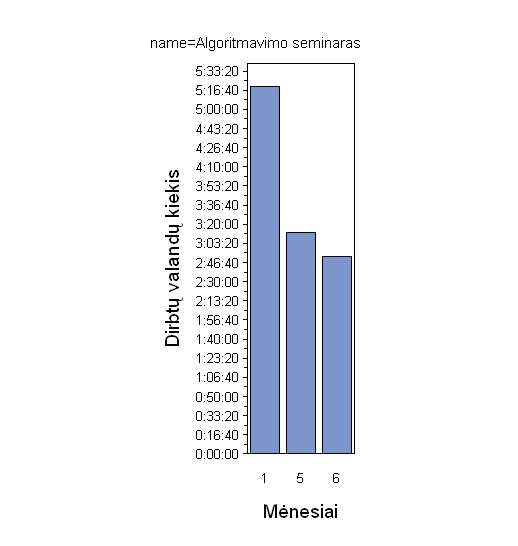
\includegraphics[width=0.3\linewidth]{%
    images/months/Algoritmavimo_seminaras.png}}
  \subfloat[Interneto technologijos]{%
    \label{fig:semester_work:interneto_technologijos}%
    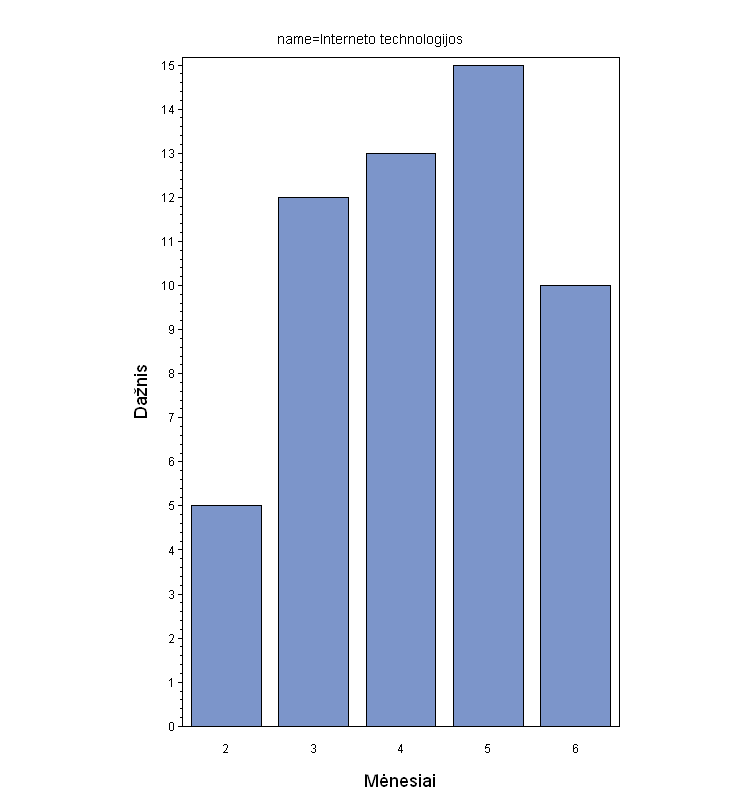
\includegraphics[width=0.3\linewidth]{%
    images/months/Interneto_technologijos.png}}
  \subfloat[Matematinė logika]{%
    \label{fig:semester_work:matematine_logika}%
    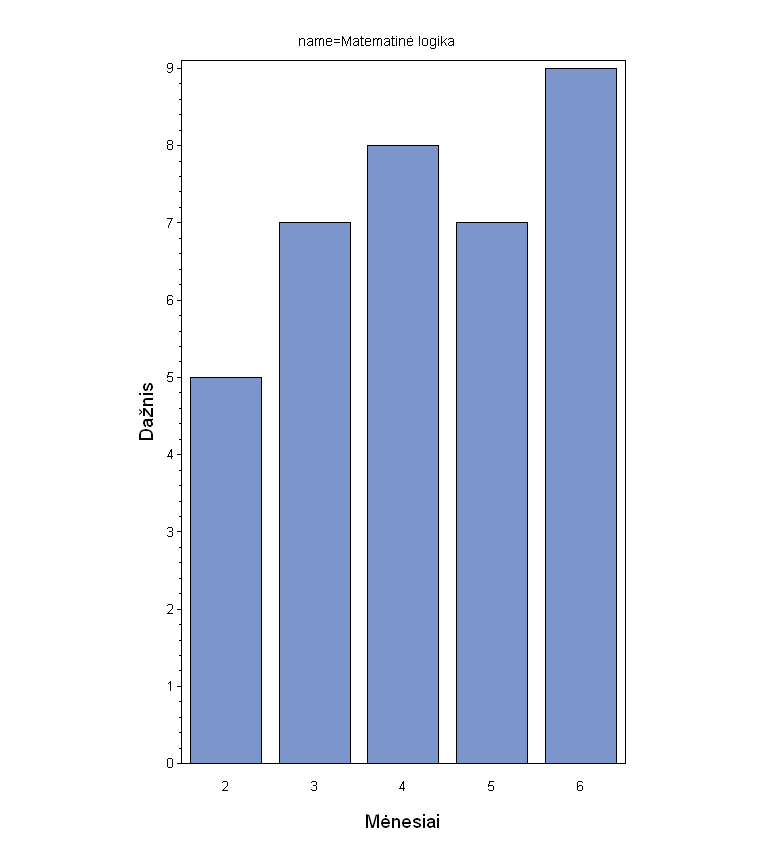
\includegraphics[width=0.3\textwidth]{%
      images/months/Matematine_logika.png}}

  \subfloat[Operacinės sistemos]{%
    \label{fig:semester_work:operacines_sistemos}%
    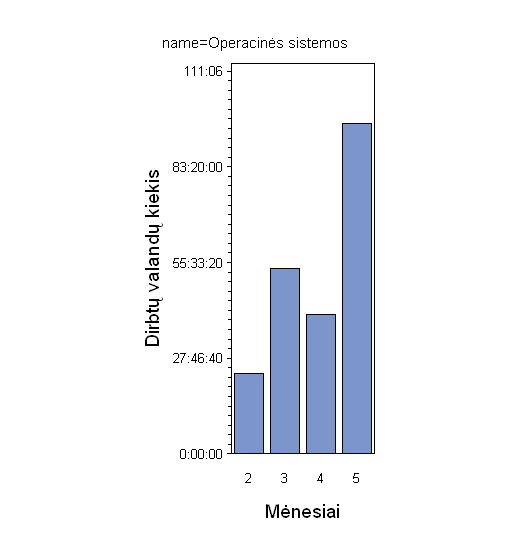
\includegraphics[width=0.3\linewidth]{%
    images/months/Operacines_sistemos.png}}
  \subfloat[Programų sistemų inžinerija]{%
    \label{fig:semester_work:programu_sistemu_inzinerija}%
    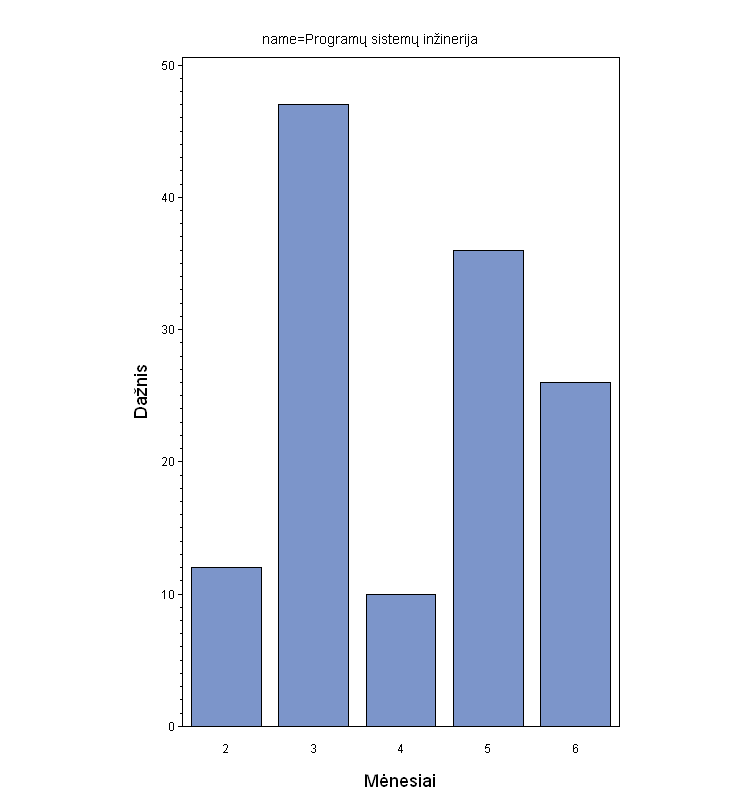
\includegraphics[width=0.3\linewidth]{%
    images/months/Programu_sistemu_inzinerija.png}}
  \subfloat[Psichologijos įvadas]{%
    \label{fig:semester_work:psichologijos_ivadas}%
    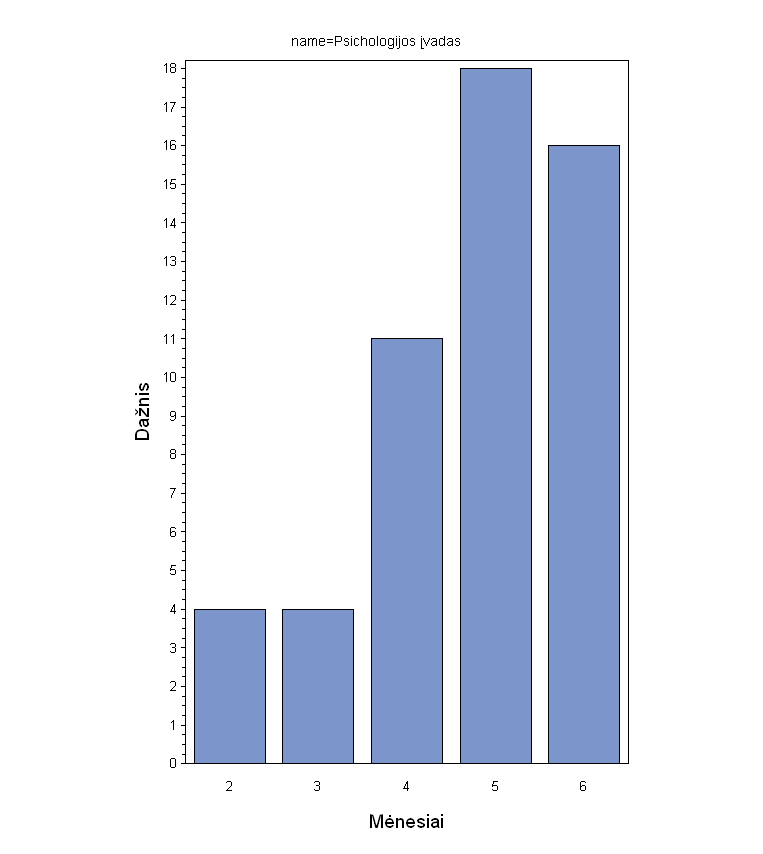
\includegraphics[width=0.3\textwidth]{%
      images/months/Psichologijos_ivadas.png}}

  \subfloat[Tikimybių teorija ir matematinė statistika]{%
    \label{fig:semester_work:tikimybiu_teorija}%
    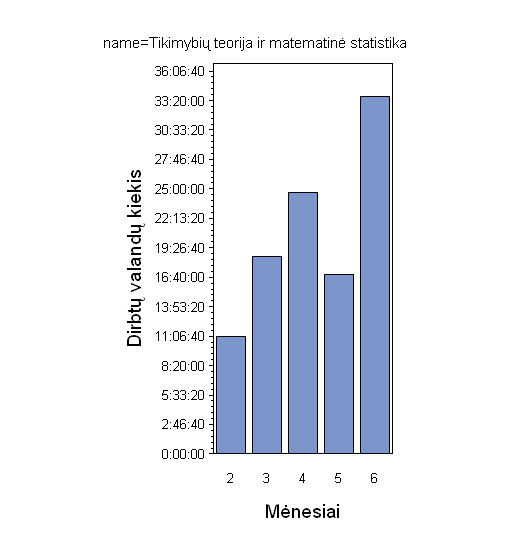
\includegraphics[width=0.3\linewidth]{%
    images/months/Tikimybiu_teorija_ir_matematine_statistika.png}}
  \subfloat[Vokiečių kalba]{%
    \label{fig:semester_work:vokieciu_kalba}%
    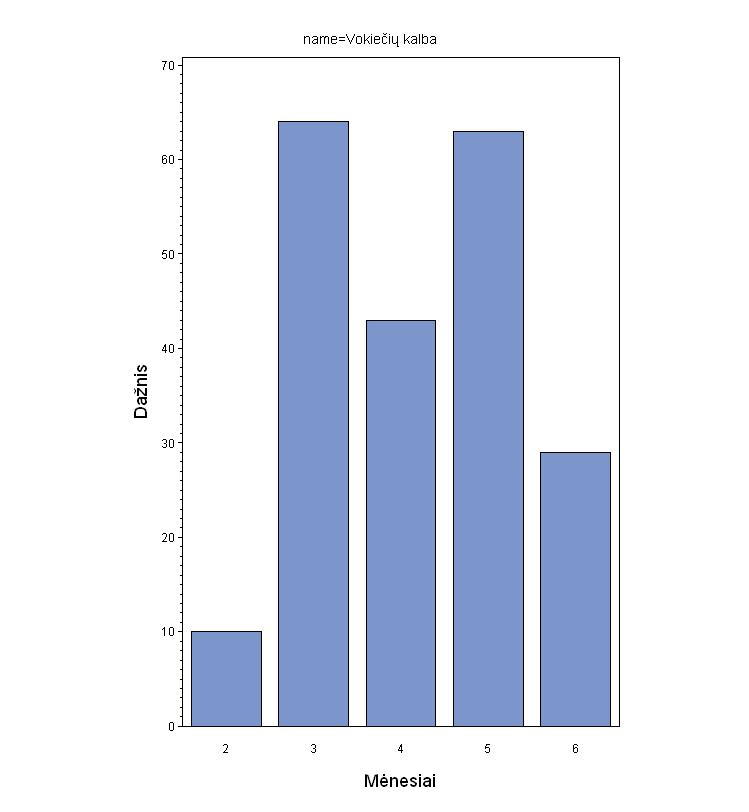
\includegraphics[width=0.3\linewidth]{%
    images/months/Vokieciu_kalba.png}}

  \caption{Darbo pasiskirstymo semestro metu analizė pagal skirtingus
    dalykus.}
  \label{fig:semester_work}
\end{figure}

\begin{listing}[H]
  \begin{minted}{splus}
  libname proj "C:\SAS\projektas\db";

/* Duomenų tvarkymas. */
data proj.visi;
format duration time8. start_date yymmdd10.;
set proj.visi;
duration=(stop_time - start_time);
month = month(start_date);
run;

/* Darbo pasiskirstymas pagal mėnesius. */
axis1 label = (a=90 height = 1.25 'Dirbtų valandų kiekis');
axis2 label = (height = 1.25 'Mėnesiai');

proc gchart data=proj.visi noprint;
vbar month /
  discrete
  sumvar=duration
  type=sum
  raxis=axis1
  maxis=axis2
  ;
by name;
run;
quit;

proc means data=proj.visi noprint;
var duration;
output out=proj.sum_month sum=sum;
by name month;
run;
  \end{minted}
  \caption{SAS programa naudota pasiskirstymų analizei.}
  \label{lst:months}
\end{listing}

\begin{sidewaystable}[ht!]
  \centering
  \begin{tabular}{|l|c|c|c|c|c|c|}
\hline
&1&2&3&4&5&6\\
Dalyko pavadinimas&sausis&vasaris&kovas&balandis&gegužė&birželis\\
\hline
Algoritmavimo seminaras&1&&&&1&1\\
Psichologijos įvadas&&0&0&0,352&0,470&1\\
Programų sistemų inžinerija&&0,379&0,608&0,102&0,665&0,936\\
Interneto technologijos&&0,154&0,139&0,220&0,243&0,769\\
Tikimybių teorija ir matematinė statistika&&0,187&0,193&0,513&0,292&0,911\\
Operacinės sistemos&&0,464&0,712&0,654&0,833&\\
Matematinė logika&&0,020&0&0,104&0&1\\
Vokiečių kalba&&0,472&0,714&0,491&0,638&0,790\\
\hline
  \end{tabular}
  \caption{Savarankiško darbo ir viso darbo santykiai.}
  \label{tab:months_part}
\end{sidewaystable}

\begin{figure}[H]
  \centering

  \subfloat[Algoritmavimo seminaras]{%
    \label{fig:semester_work_part:algoritmavimo_seminaras}%
    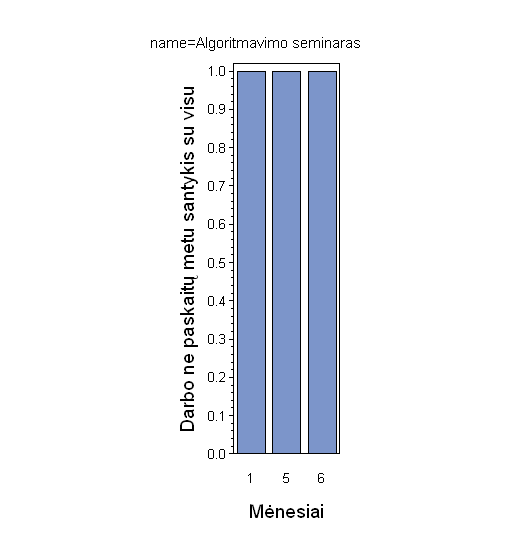
\includegraphics[width=0.3\linewidth]{%
    images/months/parts/algoritmavimo_seminaras.png}}
  \subfloat[Interneto technologijos]{%
    \label{fig:semester_work_part:interneto_technologijos}%
    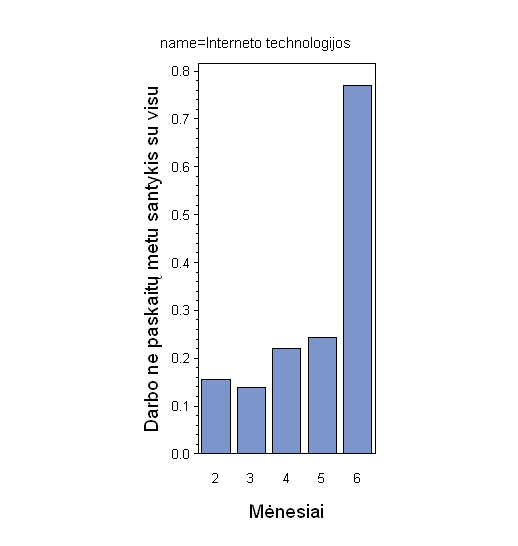
\includegraphics[width=0.3\linewidth]{%
    images/months/parts/interneto_technologijos.png}}
  \subfloat[Matematinė logika]{%
    \label{fig:semester_work_part:matematine_logika}%
    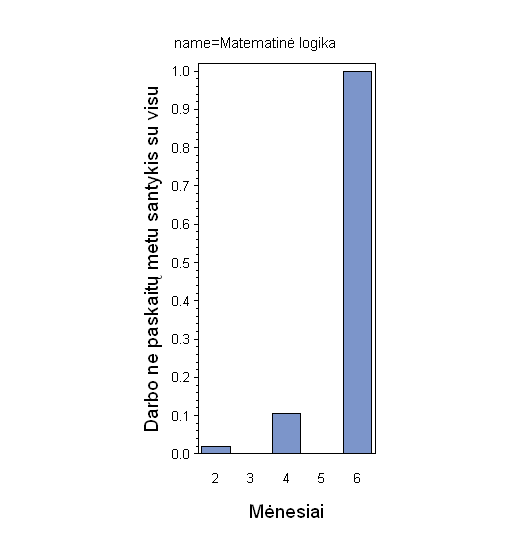
\includegraphics[width=0.3\textwidth]{%
    images/months/parts/matematine_logika.png}}

  \subfloat[Operacinės sistemos]{%
    \label{fig:semester_work_part:operacines_sistemos}%
    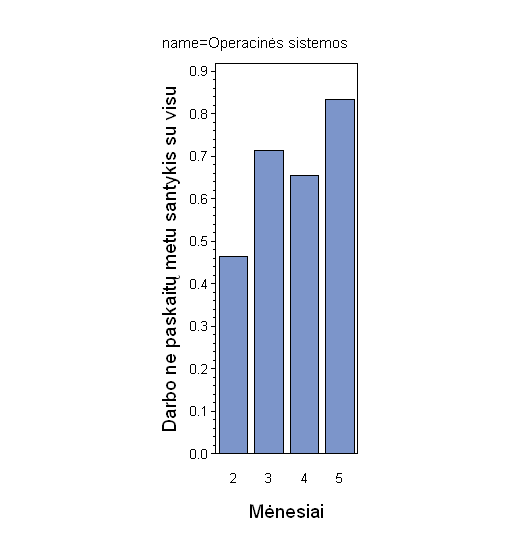
\includegraphics[width=0.3\linewidth]{%
    images/months/parts/operacines_sistemos.png}}
  \subfloat[Programų sistemų inžinerija]{%
    \label{fig:semester_work_part:programu_sistemu_inzinerija}%
    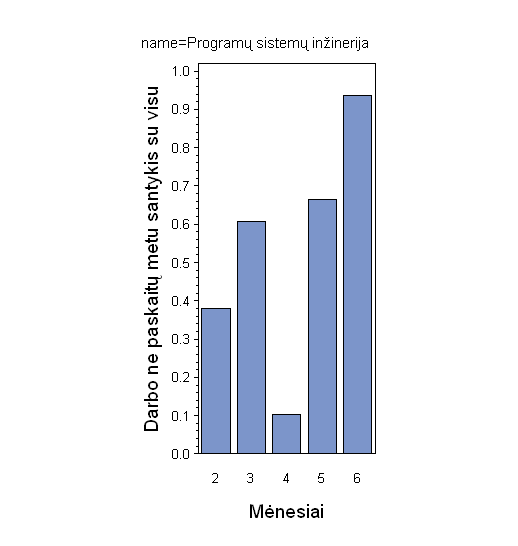
\includegraphics[width=0.3\linewidth]{%
    images/months/parts/programu_sistemu_inzinerija.png}}
  \subfloat[Psichologijos įvadas]{%
    \label{fig:semester_work_part:psichologijos_ivadas}%
    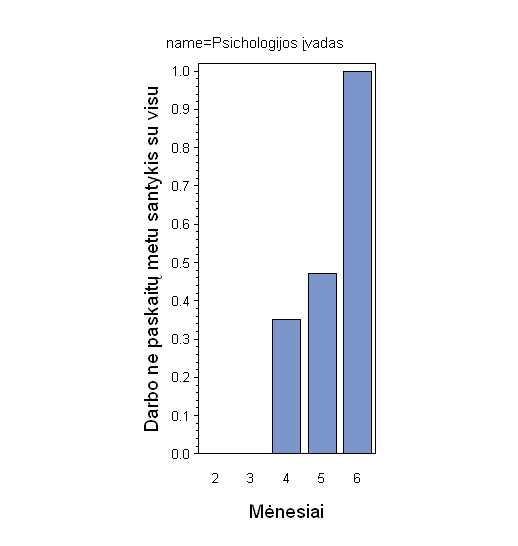
\includegraphics[width=0.3\textwidth]{%
    images/months/parts/psichologijos_ivadas.png}}

  \subfloat[Tikimybių teorija ir matematinė statistika]{%
    \label{fig:semester_work_part:tikimybiu_teorija}%
    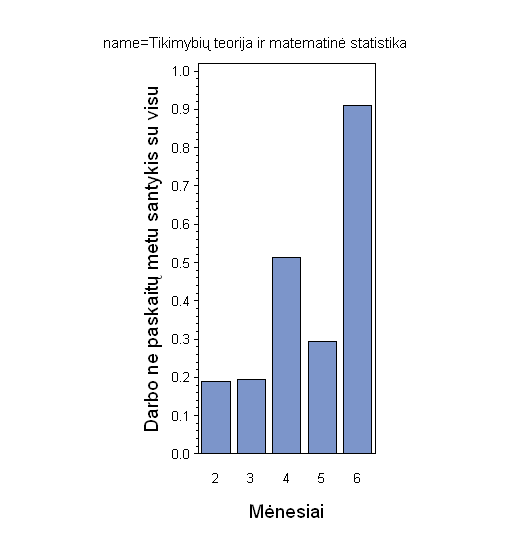
\includegraphics[width=0.3\linewidth]{%
    images/months/parts/tikimybiu_teorija_ir_matematine_statistika.png}}
  \subfloat[Vokiečių kalba]{%
    \label{fig:semester_work_part:vokieciu_kalba}%
    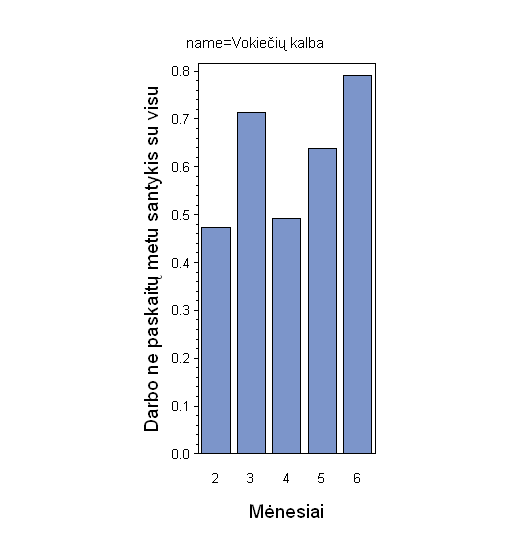
\includegraphics[width=0.3\linewidth]{%
    images/months/parts/vokieciu_kalba.png}}

  \caption{Savarankiško darbo ir viso darbo santykiai pagal mėnesius
    studijuotiems dalykams.}
  \label{fig:semester_work_part}
\end{figure}

\begin{listing}[H]
  \begin{minted}{splus}
libname proj "C:\SAS\projektas\db";

/* Duomenų tvarkymas. */
data proj.visi;
format duration time8. start_date yymmdd10.;
set proj.visi;
duration=(stop_time - start_time);
month = month(start_date);
run;

proc means data=proj.visi noprint;
var duration;
output out=proj.sum_month_all sum=all_sum;
by name month;
run;

proc means data=proj.visi noprint;
var duration;
output out=proj.sum_month_l sum=sum;
by name month;
where category_id=9;
run;

data proj.sum_month;
merge proj.sum_month_all proj.sum_month_l;
by name month;
if sum=. then sum = 0;
part = sum / all_sum;
run;

axis1 label = (
  a=90 height = 1.25
  'Darbo ne paskaitų metu santykis su visu');
axis2 label = (height = 1.25 'Mėnesiai');

proc gchart data=proj.sum_month;
vbar month / discrete sumvar=part type=sum raxis=axis1 maxis=axis2 ;
by name;
run; quit;
  \end{minted}
  \caption{SAS programa naudota santykių skaičiavimui.}
  \label{lst:months_part}
\end{listing}

\begin{figure}[H]
  \centering
    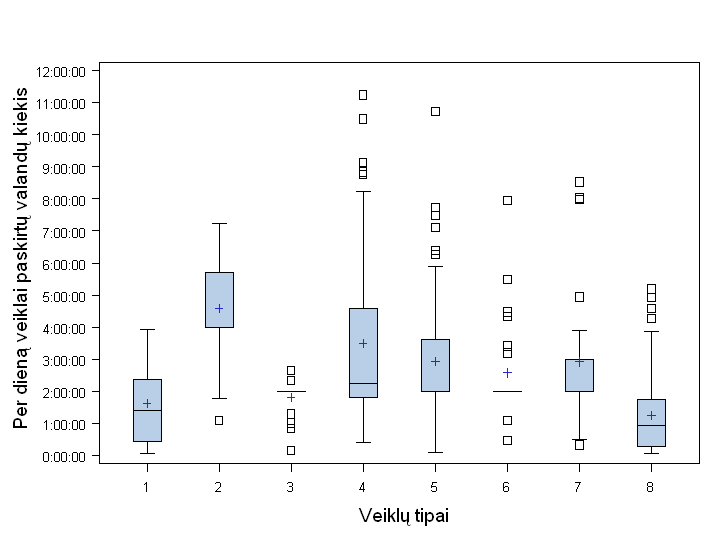
\includegraphics[width=0.9\textwidth]{images/day_duration.png}
  \caption{
    Per dieną dalykui paskirtų valandų kiekis.
    (1 – Algoritmavimo seminaras,
    2 – Interneto technologijos,
    3 – Matematinė logika,
    4 – Operacinės sistemos,
    5 – Programų sistemų inžinerija,
    6 – Psichologijos įvadas,
    7 – Tikimybių teorija ir matematinė statistika,
    8 – Vokiečių kalba)}
  \label{fig:day_duration}
\end{figure}

\begin{sidewaystable}[ht!]
  \centering
  \begin{tabular}{|p{7em}|p{4em}|c|c|c|c|c|c|c|c|}
\hline
Dalyko pavadinimas&Stebėjimų skaičius&Suma&Q1&Q2&Q3&Vidurkis&Didžiausia&Mažiausia&Nuokrypis\\
\hline
Algoritmavimo seminaras&7&11:25:00&0:26:00&1:24:00&2:22:00&1:37:51&3:56:00&0:04:00&1:18:52\\
Interneto technologijos&20&91:43:00&4:00:00&4:00:00&5:43:00&4:35:09&7:14:00&1:06:00&1:31:49\\
Matematinė logika&30&54:29:00&2:00:00&2:00:00&2:00:00&1:48:58&2:39:00&0:09:00&0:33:36\\
Operacinės sistemos&61&213:35:00&1:49:00&2:14:00&4:35:00&3:30:05&11:15:00&0:24:00&2:39:31\\
Programų sistemų inžinerija&57&166:59:00&2:00:00&2:00:00&3:37:00&2:55:46&10:44:00&0:05:00&2:02:56\\
Psichologijos įvadas&25&64:26:00&2:00:00&2:00:00&2:00:00&2:34:38&7:57:00&0:28:00&1:32:54\\
Tikimybių teorija ir matematinė statistika&36&105:01:00&1:59:30&3:00:00&3:00:00&2:55:02&8:32:00&0:20:00&1:54:38\\
Vokiečių kalba&101&125:44:00&0:17:00&0:55:00&1:44:00&1:14:42&5:12:00&0:04:00&1:12:46\\
\hline
  \end{tabular}
  \caption{Per dieną dalykui paskirtų valandų kiekio analizė.}
  \label{tab:day_duration}
\end{sidewaystable}

\begin{listing}[H]
  \begin{minted}{splus}
libname proj "C:\SAS\projektas\db";

/* Duomenų tvarkymas. */
data proj.visi;
format duration time8. start_date yymmdd10.;
set proj.visi;
duration=(stop_time - start_time);
month = month(start_date);
run;

/* Darbo pasiskirstymas pagal dienas. */
proc means data=proj.visi noprint;
var duration;
output out=proj.sum_day sum=sum;
by type_id start_date;
run;

axis1 
  order = ( 0 to 43200 by 3600)
  label = (
    height = 1.25
    'Per dieną veiklai paskirtų valandų kiekis');
axis2 label = (height = 1.25 'Veiklų tipai');

PROC BOXPLOT DATA=proj.sum_day;
PLOT sum * type_id /
  BOXSTYLE=schematic
  vaxis=axis1
  haxis=axis2;
RUN;
QUIT;
  \end{minted}
  \caption{SAS programa naudota per dieną dalykui paskirtų valandų
  diagramos braižymui.}
  \label{lst:day_duration_box}
\end{listing}

\begin{listing}[H]
  \begin{minted}{splus}
libname proj "C:\SAS\projektas\db";

/* Duomenų tvarkymas. */
data proj.visi;
format duration time8. start_date yymmdd10.;
set proj.visi;
duration=(stop_time - start_time);
month = month(start_date);
run;

proc means data=proj.visi noprint;
var duration;
output out=proj.sum_day sum=sum;
by name start_date;
run;

proc means data=proj.sum_day noprint;
var sum;
output out=proj.rez n=count sum=sum p25=q1 p50=q2 p75=q3 mean=mean
  max=max min=min std=std;
by name;
run;
  \end{minted}
  \caption{SAS programa naudota per dieną dalykui paskirtų valandų kiekio
  analizei.}
  \label{lst:day_duration_table}
\end{listing}
